\documentclass[12pt,a4paper]{article}

% ============================================================================
% Packages
% ============================================================================
\usepackage[utf8]{inputenc}
\usepackage[T1]{fontenc}
\usepackage{amsmath,amssymb}
\usepackage{graphicx}
\usepackage[margin=2.5cm]{geometry}
\usepackage{natbib}  % For citation management
\usepackage{hyperref}
\usepackage{lineno}
\linenumbers

% ============================================================================
% Document Settings
% ============================================================================
\bibliographystyle{agsm}  % Harvard style, or use 'plainnat', 'apalike', etc.
% Other common styles: abbrvnat, unsrtnat, plainnat

\title{Antarctic Bottom Water Formation Mechanisms Across Paleoclimate States: \\
Insights from Water Mass Transformation Analysis and Ventilation Age Simulations Using AWI-ESM}

\author{Your Name$^{1,2}$ and Co-authors \\
\\
\small $^1$Alfred Wegener Institute for Polar and Marine Research, Bremerhaven, Germany \\
\small $^2$Department of Geosciences, University of Bremen, Bremen, Germany}

\date{\today}

% ============================================================================
% Document Begin
% ============================================================================
\begin{document}

\maketitle

% ============================================================================
% Abstract
% ============================================================================
\begin{abstract}
Antarctic Bottom Water (AABW) is a critical component of the global meridional overturning circulation,
driving abyssal ventilation, heat storage, and carbon sequestration on centennial to millennial timescales.
Despite its importance, the mechanisms governing AABW formation across different climate states remain
poorly understood. Here we investigate AABW production during five paleoclimate periods---preindustrial (PI),
mid-Holocene (MH), Last Interglacial (LIG), Last Glacial Maximum (LGM), and Marine Isotope Stage 3 (MIS3)---using
the AWI-ESM coupled climate model. Through water mass transformation (WMT) analysis and surface buoyancy flux
decomposition using the xbudget framework, we quantify the relative contributions of thermal (longwave, shortwave,
sensible, and latent heat) and haline (sea ice and precipitation-evaporation-runoff) forcing to AABW precursor
water formation. Our results reveal a fundamental shift in formation mechanisms between climate states:
during interglacial periods (PI/MH/LIG), heat fluxes dominate AABW precursor water production (85--90\%), whereas
glacial conditions (LGM/MIS3) exhibit enhanced sea ice-driven transformation (25--30\% contribution). Surface
flux decomposition reveals that glacial conditions paradoxically \textit{reduce} ocean heat loss despite colder
atmospheric temperatures, as expanded sea ice insulates the bulk ocean while concentrating brine rejection in
coastal polynyas---a dual role that fundamentally restructures surface forcing of AABW formation. Ideal age
tracer simulations demonstrate that AABW ventilation ages during LGM/MIS3 exceed preindustrial values by
approximately 1,500 years, consistent with paleoceanographic proxy reconstructions. In contrast, the LIG Ross Sea
exhibits anomalously young ventilation ages attributed to reduced sea ice and enhanced thermal forcing. These
findings provide mechanistic insights into how sea ice governs AABW formation response to climate forcing
and contribute to understanding of deep ocean carbon storage variations across glacial-interglacial cycles.

\noindent\textbf{Keywords:} Antarctic Bottom Water, paleoclimate, water mass transformation, ventilation age, 
Southern Ocean, sea ice, Last Glacial Maximum, Last Interglacial
\end{abstract}

% ============================================================================
% Introduction
% ============================================================================
\section{Introduction}

\subsection{The critical role of Antarctic Bottom Water in the climate system}

Antarctic Bottom Water (AABW) represents the densest and coldest water mass in the global ocean, 
ventilating the abyssal ocean and playing a fundamental role in the global meridional overturning 
circulation (MOC) \citep{Orsi1999, Marshall2012}. Forming primarily around the Antarctic continental 
margin, AABW sinks to the ocean floor and spreads northward through the Atlantic, Indian, and Pacific 
basins, constituting the lower limb of the global overturning circulation \citep{Talley2013}. The 
Southern Ocean, where AABW originates, is increasingly recognized as the region where deep waters 
return to the surface through wind-driven upwelling, effectively closing the global MOC 
\citep{Marshall2012}. This dual-cell structure---with northward-flowing NADW above and 
southward-spreading AABW below---fundamentally controls the ocean's capacity to store and transport 
heat, carbon, and nutrients on centennial to millennial timescales.

The climatic significance of AABW extends far beyond its role in ocean circulation. Observations 
from repeat hydrographic sections reveal that the deep ocean below 4,000~m has accumulated heat 
at a rate of 12.9$\pm$1.8~TW since the mid-1980s, with the strongest warming signals near 
AABW source regions \citep{Purkey2010}. This abyssal warming contributes approximately 0.1~mm/yr 
to global sea level rise through thermal expansion and represents a significant component of Earth's 
energy imbalance \citep{Purkey2010}. Simultaneously, AABW has undergone substantial volume 
contraction, with the coldest and densest water classes disappearing fastest 
\citep{Purkey2012, Gunn2023}. Recent projections suggest that under high-emission scenarios, 
Antarctic meltwater could drive more than 40\% slowdown of abyssal overturning by 2050 
\citep{Li2023Nature}, with profound implications for ocean biogeochemistry and climate.

The Southern Ocean's role in the global carbon cycle is equally critical. As the primary pathway 
for deep water ventilation, the Southern Ocean mediates carbon exchange between the deep ocean 
reservoir and the atmosphere \citep{Marinov2006, Gray2024}. The Antarctic Polar Front acts as a 
biogeochemical divide, with AABW formation and sinking carrying unutilized nutrients and respired 
carbon to depth \citep{Marinov2006}. The efficiency of this biological carbon pump, and thus 
atmospheric CO$_2$ concentrations, depends sensitively on the rate and properties of AABW 
formation. The most comprehensive synthesis indicates that the Southern Ocean absorbs approximately 
40\% of oceanic anthropogenic CO$_2$ uptake, underscoring its central role in modulating 
climate change \citep{Gray2024, Rintoul2025}.

\subsection{Modern understanding of AABW formation mechanisms}

AABW formation occurs through the production and export of Dense Shelf Water (DSW) from four 
primary source regions: the Weddell Sea, Ross Sea, Adélie Coast, and Cape Darnley polynya 
\citep{Orsi1999, Ohshima2013}. The fundamental process involves transformation of surface and 
intermediate waters into extremely dense shelf waters through two interrelated mechanisms: 
intense surface heat loss and brine rejection during sea ice formation in coastal polynyas 
\citep{Silvano2023Frontiers, Ohshima2016}. High Salinity Shelf Water (HSSW) forms when 
persistent offshore katabatic winds maintain open-water polynyas, exposing the ocean surface 
to intense cooling while simultaneously enhancing sea ice production and associated brine 
rejection \citep{Miller2023, Ohshima2022}. The resulting HSSW, with salinities exceeding 
34.6~g/kg, either descends directly down the continental slope or first interacts with 
floating ice shelves to form even colder Ice Shelf Water (ISW) below $-2$°C 
\citep{Silvano2023Frontiers}.

The relative importance of thermal versus haline forcing in driving DSW formation varies 
regionally and seasonally. At Cape Darnley, intense sea ice production through frazil ice 
formation dominates, with underwater frazil penetrating depths exceeding 80~m and preventing 
heat-insulating surface ice from forming \citep{Ohshima2022}. This process enables highly 
efficient brine rejection and accounts for 6--13\% of circumpolar AABW production 
\citep{Ohshima2013}. In contrast, the Ross and Weddell Seas exhibit more complex interactions 
between polynya-driven HSSW production and ice shelf cavity circulation, with approximately 
50\% of DSW export involving ISW mixing \citep{Williams2008, Silvano2020}. Recent observations 
demonstrate that glacial meltwater input can partially offset brine injection; in the Amundsen 
Sea and Sabrina Coast, freshwater from basal melting prevents full-depth convection despite 
strong polynya activity \citep{Silvano2018}.

Climate variability strongly modulates AABW production on interannual to decadal timescales. 
The Weddell Sea has experienced a 30\% reduction in bottom water volume since 1992, 
driven primarily by more than 40\% decline in sea ice formation rates associated with northerly 
wind trends linked to the Interdecadal Pacific Oscillation \citep{Zhou2023}. Conversely, the 
Ross Sea exhibited recovery of AABW salinity, density, and thickness between 2015--2019, caused 
by anomalous wind forcing from positive Southern Annular Mode combined with extreme El Niño 
events that enhanced local sea ice formation \citep{Silvano2020}. These observations highlight 
the sensitivity of AABW production to both local surface forcing and remote climate teleconnections.

\subsection{Water mass transformation framework for AABW analysis}

The water mass transformation (WMT) framework provides a thermodynamic approach to quantifying 
how air-sea fluxes drive changes in water mass properties and thus constrain rates of dense 
water formation \citep{Walin1982, Groeskamp2019}. Originally developed by \citet{Walin1982} 
to relate surface heat fluxes to cross-isothermal mass transport, the framework was subsequently 
extended by \citet{Speer1992} to incorporate both thermal and freshwater contributions to 
surface density flux:
\begin{equation}
f_\rho = \frac{\alpha Q_{net}}{c_p} - \rho \beta S (E - P)
\end{equation}
where $\alpha$ and $\beta$ are the thermal expansion and haline contraction coefficients, 
$Q_{net}$ is the net surface heat flux, and $(E-P)$ represents net evaporation minus 
precipitation. The transformation rate across a given density surface is then obtained by 
integrating this density flux over the outcrop area \citep{Groeskamp2019}.

Modern implementations of WMT analysis decompose surface fluxes into multiple components to 
isolate specific physical processes \citep{Iudicone2008a, Iudicone2008b}. Heat flux contributions 
can be separated into shortwave radiation (accounting for penetrative effects), longwave 
radiation, sensible heat, and latent heat fluxes \citep{Iudicone2008a}. Critically, 
\citet{Iudicone2008a} demonstrated that neglecting shortwave penetration can cause 100\% 
errors in water mass formation estimates, particularly in the Southern Ocean where penetrative 
radiation affects mixed layer dynamics. Freshwater flux decomposition distinguishes between 
sea ice formation/melt, glacial meltwater, and precipitation-evaporation-runoff 
\citep{Abernathey2016, Bailey2023}. The sea ice component proves particularly important for 
AABW studies, as it acts as a ``pump'' removing freshwater from high latitudes and concentrating 
brine \citep{Abernathey2016}.

Observation-based WMT analyses have fundamentally advanced understanding of Southern Ocean 
overturning. \citet{Pellichero2018} used Argo floats, ship data, and instrumented marine 
mammals to show that seasonal sea ice growth and melt dominates water mass transformation 
in the ice-covered sector, with freshwater fluxes---rather than heat fluxes---driving the 
meridional overturning that feeds AABW formation. Their estimates indicate approximately 
27$\pm$7~Sv of deep water upwells to the surface, transforming into 22$\pm$4~Sv of lighter 
water (upper cell) and 5$\pm$5~Sv entering denser AABW classes (lower cell) 
\citep{Pellichero2018}. In the Weddell Sea specifically, closed-budget WMT analysis reveals 
minimal precipitation-evaporation-runoff contribution, with sea ice brine rejection dominating 
the surface salt flux throughout most seasons \citep{Bailey2023}.

\subsection{Why paleoclimate AABW research matters: implications for the global carbon cycle}

Understanding AABW variability across glacial-interglacial cycles is fundamental to explaining 
one of the most profound puzzles in Earth system science: the 80--100~ppm atmospheric CO$_2$ 
variations that tightly couple with temperature changes throughout the Quaternary. Ice core 
records demonstrate that CO$_2$ was among the early parameters to change at glacial terminations, 
roughly synchronous with Southern Hemisphere warming and preceding Northern Hemisphere ice 
volume decline \citep{SigmanBoyle2000}. The deep ocean, particularly the abyssal realm dominated 
by AABW, represents the primary carbon reservoir capable of explaining this magnitude of 
CO$_2$ drawdown on glacial-interglacial timescales \citep{SigmanBoyle2000, Kohfeld2005}.

The mechanistic link between AABW and atmospheric CO$_2$ operates through multiple pathways. 
Enhanced AABW formation during glacials, driven by intensified brine rejection from expanded 
sea ice, created strongly stratified deep ocean conditions that effectively isolated 
carbon-rich deep waters from atmospheric exchange \citep{Ferrari2014, Jansen2017}. Model 
studies indicate that at the Last Glacial Maximum, Antarctic-origin waters filled nearly 
the entire ocean volume below 2~km---representing approximately a fourfold increase compared 
to present---while shoaling North Atlantic Deep Water to intermediate depths 
\citep{Ferrari2014}. This reconfigured circulation trapped respired carbon at depth, with 
the Southern Ocean sea ice cap acting as an insulating lid that prevented CO$_2$ outgassing 
\citep{Ferrari2014, Marzocchi2017}. Radiocarbon evidence reveals that glacial deep ocean 
ventilation ages increased by approximately 689$\pm$53~$^{14}$C-yr compared to the Holocene, 
with southern-sourced abyssal waters particularly isolated \citep{Skinner2017}. This 
enhanced isolation could account for more than 50\% of the observed 80--100~ppm glacial 
CO$_2$ drawdown \citep{Skinner2017}.

Beyond its role in glacial CO$_2$ storage, AABW behavior during past warm periods provides 
crucial insights for projecting future climate trajectories. During Marine Isotope Stage 4 
(MIS4; $\sim$70--60~ka), atmospheric CO$_2$ decreased by approximately 40~ppm within 
several thousand years, driven by multiple carbon cycle mechanisms including enhanced AABW 
formation and export that strengthened deep ocean carbon storage \citep{Baggenstos2019}. 
Conversely, interglacial AABW weakening events---as documented during the Last Interglacial 
\citep{Hayes2014} and recurrent across multiple interglacials \citep{Glasscock2020}---demonstrate 
the sensitivity of deep ocean ventilation to high-latitude freshwater forcing. These past 
analogs are particularly relevant given projections of substantial Antarctic ice sheet mass 
loss and associated meltwater discharge under future warming scenarios \citep{Li2023Nature}.

The paleoclimate perspective is essential because the modern instrumental record provides 
insufficient temporal scope to evaluate climate model performance on centennial-to-millennial 
timescales \citep{ZhouWEA2016, Tierney2020Paleo}. The climate system is far from equilibrium 
within the $\sim$150-year observational period, limiting our ability to constrain equilibrium 
climate sensitivity and assess long-term climate feedbacks \citep{Sherwood2020}. Paleoclimate 
states spanning dramatically different CO$_2$ levels, ice sheet configurations, and ocean 
circulation patterns provide ``out-of-sample'' tests for models developed primarily using 
modern observations \citep{Zhu2021NCC}. For AABW specifically, paleoclimate constraints 
offer the only means to evaluate how formation mechanisms respond to forcing changes 
spanning full glacial-interglacial amplitudes.

\subsection{State of paleoclimate AABW research: proxy records and modeling advances}

\subsubsection{Proxy-based reconstructions of past AABW variability}

Multiple geochemical tracers have been developed to reconstruct past AABW properties and 
circulation pathways. Benthic foraminiferal $\delta^{13}$C has been extensively applied as 
a quasi-conservative water mass tracer, exploiting the distinct isotopic signatures of NADW 
(high $\delta^{13}$C from nutrient-depleted source waters) versus AABW (low $\delta^{13}$C 
from incomplete surface nutrient utilization) \citep{Curry1988, OppoFairbanks1987}. Compilations 
of benthic $\delta^{13}$C from the Atlantic reveal a dramatic restructuring at the LGM, with 
NADW shoaling to intermediate depths ($\sim$2,000~m) and AABW expanding to fill the abyssal 
Atlantic \citep{Curry2005, Hines2021}. However, $\delta^{13}$C is influenced by both circulation 
and biogeochemistry (air-sea gas exchange, biological productivity, respiration), complicating 
interpretation \citep{Eide2017}.

Neodymium isotopes ($\epsilon_{Nd}$) have emerged as a powerful quasi-conservative tracer 
for reconstructing deep water mass geometry \citep{Goldstein2003, Piotrowski2005}. Modern 
observations show NADW characterized by unradiogenic $\epsilon_{Nd}$ values ($\sim$-13), 
whereas AABW and Pacific deep waters display more radiogenic signatures ($\sim$-8 to -7) 
\citep{Lacan2005, Lambelet2016}. High-resolution $\epsilon_{Nd}$ records spanning the last 
glacial cycle demonstrate oscillating NADW and AABW contributions to deep Atlantic ventilation, 
with AABW influence maximized during stadials and Heinrich events \citep{Piotrowski2008, 
Huang2020}. Recent modeling studies incorporating neodymium cycling confirm that $\epsilon_{Nd}$ 
variations primarily reflect changes in NADW versus AABW formation rates and mixing patterns, 
with boundary exchange processes as the dominant Nd source \citep{Gu2019, Poppelmeier2022}.

Radiocarbon-based ventilation ages provide the most direct constraint on deep ocean circulation 
rates. Benthic-planktonic (B-P) $^{14}$C age offsets reveal globally increased deep ocean 
isolation during glacials, with the most extreme values in the deep Pacific and Southern Ocean 
\citep{Broecker1984, Skinner2010}. However, methodological refinements demonstrate that bulk 
B-P ages comprise both circulation age and ``preformed $^{14}$C-age'' arising from incomplete 
atmosphere-ocean equilibration at formation regions---particularly problematic in the sea 
ice-covered Southern Ocean \citep{Koeve2015}. Recent deglacial reconstructions reveal a 
``radiocarbon ventilation seesaw,'' with deep Pacific and Atlantic ventilation ages changing 
in opposite phases, explained by alternating NADW versus AABW production \citep{Skinner2014, 
Skinner2021}. Transient simulations using ideal age tracers demonstrate that true (ideal) 
ventilation age was modestly younger at the LGM compared to present due to stronger AABW 
transport from enhanced brine rejection, reconciling the apparently contradictory radiocarbon 
evidence \citep{Li2024CP}.

Additional proxies provide complementary constraints. Authigenic uranium (aU) records detect 
deep ocean oxygenation changes, with reduced aU accumulation indicating decreased bottom 
water oxygenation during AABW weakening events \citep{Hayes2014, Glasscock2020}. Benthic 
$^{231}$Pa/$^{230}$Th ratios constrain meridional overturning intensity, though interpretation 
is complicated by boundary scavenging effects \citep{Negre2010, Lippold2016}. Benthic 
foraminiferal $\delta^{18}$O and Mg/Ca jointly constrain deep ocean temperature and salinity 
evolution \citep{Adkins2002, Elderfield2012}, revealing that the glacial deep ocean was 
near freezing point globally with the Southern Ocean containing the saltiest deep water 
(37.1~psu) \citep{Adkins2002}.

\subsubsection{Modeling studies of AABW across paleoclimate states}

Paleoclimate modeling has advanced from simplified box models \citep{Toggweiler1999, 
Gildor2001} through intermediate complexity models \citep{Menviel2012, Bouttes2012} to 
comprehensive Earth System Models participating in the Paleoclimate Modelling Intercomparison 
Project (PMIP) \citep{Braconnot2012, Kageyama2017}. Early studies using conceptual models 
identified key mechanisms linking Southern Ocean processes to atmospheric CO$_2$: enhanced 
stratification reducing CO$_2$ outgassing \citep{Francois1997, Toggweiler1999}, equatorward 
wind shifts reducing upwelling of CO$_2$-rich waters \citep{Toggweiler2006}, and expanded 
sea ice capping deep waters \citep{Stephens2000}.

Comprehensive model intercomparisons under PMIP3/CMIP5 revealed substantial inter-model 
spread in simulated glacial ocean circulation changes \citep{Weber2007, Marzocchi2019}. 
Some models show weakened Atlantic overturning at the LGM, while others maintain vigorous 
circulation \citep{Weber2007}. The representation of Antarctic sea ice varies dramatically, 
with PMIP3 models showing September sea ice extent ranging from 10--30$\times10^6$~km$^2$ 
compared to proxy-based estimates of $\sim$17$\times10^6$~km$^2$ \citep{Lhardy2022}. These 
discrepancies propagate to simulated deep ocean ventilation and carbon storage.

Recent advances include transient deglacial simulations that capture temporal evolution 
of circulation changes. The TRACE-21ka simulation demonstrates that AABW transport variations 
primarily control global deep ocean ventilation age, with ages peaking at 1,900--2,200~years 
around 14--12~ka during weakened AABW transport \citep{Liu2009, Li2024CP}. Isotope-enabled 
simulations (e.g., iLOVECLIM, iCESM) now incorporate radiocarbon, stable isotopes, and trace 
elements, enabling direct model-data comparison using the same tracers measured in proxy 
records \citep{Menviel2017, Gu2019, Poppelmeier2022}. These developments allow quantitative 
assessment of whether models capture first-order circulation changes indicated by proxy 
compilations.

Despite progress, fundamental limitations persist. As discussed earlier, most CMIP6 models 
form AABW through open-ocean deep convection rather than realistic shelf processes 
\citep{Heuze2021}. This affects not only the spatial distribution of formation but potentially 
the sensitivity of AABW to climate forcing. Resolution constraints prevent explicit 
representation of critical small-scale processes: coastal polynyas ($\sim$10--100~km), 
dense water cascades down continental slopes, and ice shelf cavity circulation 
\citep{Schmidt2025}. Parameterizations attempt to compensate but introduce additional 
uncertainties and tuning requirements \citep{Dufour2017}.

\subsubsection{Model-data comparison challenges and uncertainties}

Quantitative model-data comparison faces multiple obstacles. Proxy records and model outputs 
represent fundamentally different quantities: proxies measure geochemical tracers integrated 
over specific time windows, whereas models directly simulate physical variables 
\citep{Phipps2013, Evans2013}. Proxy System Models (PSMs) provide a framework for translating 
model output into proxy space, but PSM uncertainties can be substantial \citep{Evans2013, 
Dee2015}. For instance, benthic foraminiferal $\delta^{18}$O reflects both temperature and 
seawater $\delta^{18}$O (itself influenced by salinity, ice volume, and local hydrology), 
requiring multi-proxy approaches or model-derived seawater $\delta^{18}$O fields to isolate 
temperature \citep{Rohling1998}.

Chronological uncertainties pose additional challenges, particularly for integrating records 
across multiple sites. Radiocarbon dating uncertainties of $\pm$100--300~years are typical 
for the last glacial period, with larger uncertainties for older periods or in archives with 
low carbonate content \citep{Reimer2020}. Reservoir age corrections for marine radiocarbon 
introduce further uncertainty, particularly where past reservoir ages differed from modern 
\citep{Skinner2019}. These age uncertainties complicate identification of lead-lag relationships 
and assessment of synchroneity between different regions or climate components.

Spatial coverage remains limited. High-quality proxy records concentrate in specific regions 
(North Atlantic, Southern Ocean sectors) with large data gaps elsewhere. The deep Pacific, 
which contains $\sim$50\% of ocean volume, has relatively sparse coverage \citep{Skinner2019}. 
This spatial heterogeneity challenges global synthesis efforts and means model-data comparisons 
rely heavily on regional patterns that may not represent global-scale changes.

Recent efforts have improved these challenges through coordinated data synthesis initiatives 
(e.g., MARGO for LGM sea surface temperatures \citep{MARGO2009}, LGMNd isotope compilation 
\citep{Piotrowski2012}), standardized model-data comparison metrics \citep{Hargreaves2011, 
Kageyama2021}, and paleoclimate data assimilation techniques that formally combine proxy 
information with model simulations while accounting for respective uncertainties 
\citep{Tierney2020Paleo, Osman2021}. Despite progress, model-data consistency varies 
substantially across variables and regions, with models often underestimating the magnitude 
of reconstructed regional changes \citep{Harrison2012}.

\subsection{Knowledge gaps and research objectives}

Despite substantial progress, several critical gaps constrain our understanding of AABW 
formation mechanisms across paleoclimate states. First, \textbf{the relative importance of 
thermal versus haline forcing in AABW precursor water formation has not been systematically 
quantified across multiple climate states using consistent methodology}. While modern 
observations and reanalysis-driven water mass transformation analyses have illuminated 
contemporary formation mechanisms \citep{Pellichero2018, Bailey2023}, comparable analysis 
across glacial and interglacial climates remains absent. The limited studies that exist 
focus on single climate states or employ different methodological approaches, precluding 
robust inter-period comparison.

Second, \textbf{mechanistic understanding of regional differences in AABW response to climate 
forcing requires further investigation}. Why does the Ross Sea exhibit particularly young 
ventilation ages during the LIG despite other Southern Ocean regions showing slightly older 
ages? What controls the spatial distribution of AABW formation intensity changes between 
glacial and interglacial periods? These regional variations likely reflect complex interactions 
between sea ice dynamics, ice shelf geometry, bathymetry, and atmospheric forcing, but 
systematic analysis linking surface forcing to formation rate changes across source regions 
is lacking.

Third, \textbf{model-simulated ventilation ages have not been comprehensively validated 
against proxy reconstructions across the full spectrum of warm and cold climate states}. 
Most model-data radiocarbon comparisons focus on the LGM and deglaciation \citep{Menviel2017, 
Li2024CP}, with fewer studies examining interglacial periods including the LIG and 
mid-Holocene. Given evidence for distinct AABW behavior during warm versus cold periods 
\citep{Hayes2014, Ferrari2014}, systematic validation across this full range is essential 
for assessing whether models capture first-order circulation physics.

Fourth, \textbf{the implications of model limitations in representing AABW formation processes 
remain poorly quantified}. While it is recognized that most models form AABW through 
open-ocean deep convection rather than shelf overflows \citep{Heuze2021, deLavergne2014}, 
the consequences for paleoclimate applications are unclear. Does incorrect formation 
mechanism compromise the models' ability to simulate AABW's response to forcing? Under 
what circumstances might models still provide useful insights despite this limitation? 
Some evidence suggests relative changes may be more robust than absolute values 
\citep{Menviel2021CP}, but systematic evaluation is lacking.

Finally, \textbf{integrated analysis combining mechanistic process studies, tracer-based 
validation, and systematic comparison across multiple climate states is rare}. Most studies 
focus on single aspects: circulation changes OR carbon cycle implications OR specific 
formation mechanisms. Comprehensive studies that link surface forcing $\rightarrow$ water 
mass transformation $\rightarrow$ AABW properties $\rightarrow$ ventilation changes 
$\rightarrow$ biogeochemical impacts across multiple climate states would provide crucial 
mechanistic insights.

This study addresses these gaps through systematic water mass transformation analysis and 
ventilation age diagnostics across five carefully selected paleoclimate periods spanning 
glacial and interglacial conditions. By decomposing surface buoyancy fluxes into individual 
thermal and haline components, we quantify how the dominant driver of AABW precursor water 
formation shifts between climate states. Ideal age tracer simulations enable comparison 
with radiocarbon-based proxy reconstructions, validating the model's representation of 
circulation changes. While acknowledging that our model, like most climate models, produces 
AABW through open-ocean convection rather than fully realistic shelf processes, we demonstrate 
that comparative analysis across climate states reveals robust mechanistic patterns. These 
results illuminate fundamental controls on deep ocean ventilation and carbon storage across 
glacial-interglacial cycles, providing process-level insights essential for understanding 
past climate variations and projecting future deep ocean changes.

\subsection{Model representation challenges}

Climate models face systematic challenges in representing AABW formation. Comprehensive 
assessment of CMIP6 models reveals that 28 out of 35 models form AABW predominantly through 
open-ocean deep convection rather than realistic shelf overflow processes \citep{Heuze2021}. 
This limitation stems primarily from insufficient horizontal resolution to resolve shelf 
processes, which require approximately 2--4~km resolution \citep{Schmidt2025}. However, 
recent model developments show promising improvements \citep{Mohrmann2021}, and models 
with overflow parameterizations can achieve accurate AABW properties even at coarse resolution 
\citep{Schmidt2025}. Despite these limitations, paleoclimate model studies remain valuable 
when constraints are properly acknowledged, as relative changes in response to forcing may 
be robust even when absolute values contain biases \citep{Menviel2021CP, Zhu2025}.

% Continue with more subsections...

% ============================================================================
% Methods (example section)
% ============================================================================
\section{Methods}

\subsection{Model description and experimental design}


The model used in this study, AWIESM2, is a state-of-the-art Earth system model developed at the Alfred Wegener Institute (AWI) \citep{sidorenko2019evaluation}. It consists of an atmospheric component, ECHAM6 \citep{stevens2013atmospheric},  which includes a land-surface component JSBACH representing dynamic vegetation with two types of bare surface and multiple plant functional types \citep{brovkin2009global,reick2013representation,reick2021jsbach}, as well as an ice-ocean model FESOM2 employing a multi-resolution dynamical core based on finite volume formulation \citep{danilov2017finite}. The atmosphere grid applied in the present study is T63L47, which has a global mean spatial resolution of 1.875° with 47 vertical levels.  A spatially-variable resolution is used for the ice-ocean component (Fig. S1), from about 100 km in the open ocean to 25 km over polar areas and 35 km for the equatorial belt and along coastlines. Vertically, there are 46 uneven layers in the ocean. 

% Continue with your methods...
We perform 5 equilibrium simulations, representing 3 interglacial time periods, i.e., pre-industrial (PI), mid-Holocene (MH), and last interglacial (LIG), as well as 2 glacial periods, i.e., Last Glacial Maximum (LGM) and Marine Isotope Stage 3 (MIS3).  The initial conditions for the atmosphere in our PI simulation are derived from the Atmospheric Model Intercomparison Project (AMIP) \citep{roeckner2004atmospheric}. The ocean model is initialized with the  World Ocean Atlas (WOA)  climatological temperature and salinity data for the years 1950-2000 \citep{levitus2010world}. We run the PI simulation for 1,500 model years with dynamic vegetation. The MH and LIG simulations are initialized from the PI run. The boundary conditions are configured following the criteria of PMIP4 \citep{otto2017pmip4}. Orbital parameters are calculated following \citet{berger1977long}, and the greenhouse gas concentrations are taken from multi-archive reconstructions from ice core records and recent measurements of firn air and atmospheric samples \citep{fluckiger2002high,monnin2004evidence,schilt2010glacial,buiron2011taldice,schneider2013reconstruction,kohler2017156}.
The CO$_2$ concentration used in our study is 284.32 ppm for PI, 264.4 ppm for MH, 275 ppm for LIG, 210.5 ppm for MIS3, and 190 ppm for LGM. For LGM and MIS3, we fix the boundary conditions at 21 ka and 38 ka respectively. The topography and ice-sheet properties are derived from the GLAC1D reconstruction  \citep{tarasov2003greenland,tarasov2012data,briggs2014data}. Both LGM and MIS3 experiments are initialized from a previous LGM model study \citep{werner2016glacial}. All of the 4 paleo simulations are integrated for  1,000 model years, with the simulated climate  being in a quasi-equilibrium state for the final 100 model years.

\subsection{Surface buoyancy flux decomposition using xbudget}

To quantify the individual contributions of different physical processes to surface buoyancy forcing, we employ the xbudget Python package (https://github.com/hdrake/xbudget), which provides model-agnostic tools for analyzing finite-volume ocean model budgets \citep{xbudget2024}. The xbudget framework, built on xarray and xgcm, enables systematic decomposition of tracer budgets into individual forcing terms while maintaining numerical consistency with the underlying model's finite-volume discretization.

We compute surface density tendency budgets for three tracers (mass, heat, and salt) following the MOM6 surface budget configuration. For each experiment, monthly climatological output from FESOM2 is first regridded from the unstructured mesh to a regular 0.5°×0.5° latitude-longitude grid using pyfesom2's nearest-neighbor interpolation with 80-km search radius. ECHAM6 surface fluxes (shortwave radiation var95, longwave radiation var92, latent heat var111, sensible heat var120) are interpolated to the ocean grid using scipy's griddata method. Freshwater fluxes include precipitation (prlq), snowfall (prsn), evaporation (evs), river runoff (friver), and sea ice melt/formation (fsitherm), with sea ice freshwater flux assumed to have salinity S$_{ice}$ = 5~psu.

The xbudget analysis decomposes surface density tendency into:
\begin{equation}
\frac{\partial \rho}{\partial t}\bigg|_{\text{surface}} = \frac{\partial \rho}{\partial t}\bigg|_{\text{mass}} + \frac{\partial \rho}{\partial t}\bigg|_{\text{heat}} + \frac{\partial \rho}{\partial t}\bigg|_{\text{salt}}
\end{equation}

For heat flux decomposition, we run xbudget five times with different heat flux configurations (total, shortwave only, longwave only, latent heat only, sensible heat only), setting non-selected components to zero in each run. This isolates the individual contribution of each heat flux component to surface density tendency. The salt budget similarly decomposes freshwater forcing into individual precipitation, evaporation, sea ice, runoff, and snowfall contributions. All budget terms are output in units consistent with FESOM2's tracer equations: heat (W~m$^{-2}$), mass (kg~m$^{-2}$~s$^{-1}$), and salt (psu~s$^{-1}$).

We analyze both austral winter (JJA: June-July-August) and summer (DJF: December-January-February) seasonal means to assess the year-round persistence of identified mechanisms. Sea ice masks are applied to brine rejection terms, setting them to zero where monthly sea ice concentration falls below threshold (a$_{ice}$ = 0). Spatial patterns are smoothed using a Gaussian filter (σ = 1.5 grid points) to reduce small-scale noise while preserving large-scale structure.

\subsection{Water mass transformation analysis using xwmt}

Water mass transformation (WMT) analysis provides a quantitative framework for diagnosing formation rates of water masses in density coordinates, following the approach of \citet{Walin1982} and \citet{Groeskamp2019}. We employ the xwmt Python package (https://github.com/NOAA-GFDL/xwmt), an xarray-based framework developed at NOAA-GFDL specifically designed for calculating water mass transformations in a computationally efficient manner \citep{xwmt2024}.

The xwmt package implements the Walin water mass transformation framework, which relates surface buoyancy fluxes to the formation rate of water masses in density space. For a given density class σ, the transformation rate $G$(σ) represents the volume flux (in Sverdrups, 1~Sv = 10$^6$~m$^3$~s$^{-1}$) across that density surface due to surface forcing. Positive $G$(σ) indicates water becoming denser through surface buoyancy loss, while negative $G$(σ) indicates lightening through buoyancy gain.

The total transformation is decomposed into contributions from individual forcing components:
\begin{equation}
G_{\text{total}}(\sigma) = G_{\text{heat}}(\sigma) + G_{\text{salt}}(\sigma)
\end{equation}
where $G_{\text{heat}}$ represents transformation due to surface heat fluxes and $G_{\text{salt}}$ captures haline forcing from freshwater fluxes. The salt component is further decomposed into sea ice contributions (brine rejection and melt) and other freshwater sources (precipitation, evaporation, runoff, snowfall).

For each paleoclimate experiment, we compute WMT in four key Southern Ocean regions: (1) Southern Ocean (south of 60°S), (2) Ross Sea (180°W--60°W), (3) Weddell Sea (60°W--79°E), and (4) Ad\'elie Land (79°E--180°E). These regions encompass the primary AABW formation sites and allow regional comparison of formation mechanisms. Regional transformations are calculated by applying spatial masks to the areacello-weighted surface forcing fields before integration.

The computational workflow integrates xbudget and xwmt seamlessly. After xbudget decomposes surface forcing into individual heat and salt components (Section 2.2), these decomposed budgets are passed directly to xwmt's WaterMassTransformations class. The xwmt framework constructs an xgcm Grid object that handles metric terms (cell areas) and boundary conditions for proper spatial integration. Transformations are computed in σ$_2$ (potential density referenced to 2000~dbar) space using 0.1~kg/m$^3$ bins spanning σ$_2$ = 0--40~kg/m$^3$, with dense water formation (σ$_2$ $>$ 36.5~kg/m$^3$) as the primary focus.

We analyze both annual mean and austral winter (JJA) transformation rates, as AABW formation exhibits strong seasonal modulation. Winter transformations typically exceed annual means by factors of 2--3 due to enhanced convection and sea ice formation during the cold season. The xwmt package's lazy evaluation strategy (leveraging Dask) enables efficient processing of high-resolution unstructured mesh data across multiple experiments and configurations without exceeding memory constraints.

% ============================================================================
% Results (example structure)
% ============================================================================
\section{Results}

\subsection{Large-scale features of the Southern Ocean}

The simulated JJA (austral winter) climate patterns reveal distinct characteristics across the five paleoclimate states (Fig.~1--3). SST anomalies relative to PI exhibit strong regional contrasts: LIG shows pronounced warming ($>$2°C) in the Bellingshausen-Amundsen Seas, while LGM and MIS3 display basin-wide cooling exceeding 5°C. SSS anomalies follow similar spatial patterns, with LIG freshening and glacial periods showing widespread salinification (up to 2~psu) driven by expanded sea ice. Density ($\sigma_2$) changes reflect combined thermal and haline effects, with glacial periods exhibiting substantially denser surface waters ($\Delta\rho >$~0.6~kg/m$^3$) particularly in the Atlantic and Indian sectors.

Sea ice extent and MLD exhibit the most dramatic inter-period differences (Fig.~2). Glacial simulations show circumpolar sea ice coverage extending to $\sim$50°S, while LIG displays reduced ice extent compared to PI, particularly in the Ross and Weddell Seas. Winter MLD reaches 200--400~m in PI/MH/LIG polynyas but exceeds 500~m in glacial Atlantic sector, consistent with enhanced convection.

Wind patterns reveal systematic shifts (Fig.~3). The westerly wind maximum strengthens and shifts poleward in LIG, generating positive wind speed anomalies south of 55°S. Conversely, LGM and MIS3 exhibit equatorward-shifted, weakened westerlies. Wind stress anomalies mirror these patterns, with LIG showing enhanced Southern Ocean wind stress ($\Delta\tau >$~0.04~N/m$^2$) in the 50--60°S band, while glacial periods display widespread stress reduction. These atmospheric circulation changes directly modulate Ekman upwelling and polynya ventilation efficiency.

\subsection{Surface buoyancy flux decomposition}

To understand the physical processes driving water mass transformation, we decompose surface buoyancy fluxes into their individual heat and freshwater components using the xbudget framework (Section 2.3). This analysis isolates how different atmospheric and oceanic processes contribute to surface density changes that ultimately drive AABW formation.

\subsubsection{Heat flux patterns and the sea ice insulation paradox}

During the preindustrial period (Fig.~4a,f,k), the Southern Ocean experiences strong circumpolar heat loss to the atmosphere, with total heat flux reaching $-$0.2 to $-$0.1~kJ~s$^{-1}$~m$^{-2}$ in austral winter (JJA). This cooling is dominated by turbulent heat fluxes (latent and sensible heat; Fig.~4k) rather than radiative components (shortwave and longwave; Fig.~4f), reflecting the importance of ocean-atmosphere turbulent exchange in driving surface densification. The strongest heat loss occurs in the Weddell and Ross Seas and along the coastal polynya regions where persistent offshore winds expose ocean surfaces to frigid atmospheric conditions.

Interglacial climate anomalies (MH, LIG) show minimal heat flux changes in most regions, with MH exhibiting nearly neutral anomalies (Fig.~4b,g,l) and LIG displaying localized warming in the Ross Sea sector (reduced heat loss of $\sim$0.1~kJ~s$^{-1}$~m$^{-2}$; Fig.~4c). This Ross Sea anomaly reflects reduced sea ice coverage during LIG, allowing enhanced ocean-atmosphere heat exchange in a region that remains ice-covered during PI winter.

Glacial periods (LGM, MIS3) reveal a counterintuitive phenomenon: despite substantially colder atmospheric temperatures, the ocean experiences \textit{reduced} heat loss compared to PI (Fig.~4d,e). Heat flux anomalies of +0.1 to +0.2~kJ~s$^{-1}$~m$^{-2}$ (blue colors indicating less cooling) appear throughout the Southern Ocean, with both radiative (Fig.~4i,j) and turbulent (Fig.~4n,o) components contributing to this effect. Critically, the turbulent flux reduction \textit{exceeds} the radiative reduction, indicating that the physical mechanism involves blocking ocean-atmosphere exchange rather than changes in radiative forcing alone.

This \textbf{sea ice insulation paradox}---warmer ocean surfaces (less heat loss) despite colder air---arises from expanded glacial sea ice acting as a thermal insulating lid. The ice cover prevents turbulent heat exchange (evaporation and sensible heat loss) more effectively than it blocks radiation, fundamentally altering the surface energy balance. During summer (DJF; Fig.~5), this insulation effect weakens but persists in the glacial ice-covered sectors, demonstrating that sea ice's thermal role operates year-round albeit with seasonal modulation. The summer patterns (Fig.~5) show reduced anomaly magnitudes but similar spatial structures, confirming that the insulation mechanism is intrinsic to ice cover rather than a winter-only phenomenon.

\subsubsection{Freshwater flux patterns and coastal brine intensification}

Surface freshwater fluxes, which drive haline forcing of density, exhibit starkly different patterns (Fig.~6--7). The PI baseline (Fig.~6a,f,k) shows modest total freshwater fluxes, with coastal regions experiencing brine rejection during sea ice formation (red colors in Fig.~6f indicating surface salinification) and offshore zones receiving freshwater from ice melt (blue colors). Other freshwater sources (precipitation, evaporation, runoff, snowfall; Fig.~6k) contribute weak net effects in winter.

Glacial periods transform this pattern dramatically. Total freshwater flux anomalies (Fig.~6d,e) reveal strong positive values (blue: net freshwater gain) along the Antarctic coast, but this bulk signal masks opposing contributions from different components. The sea ice component (Fig.~6i,j) shows \textit{intensified} coastal brine rejection (red: +0.0002~kg~s$^{-1}$~m$^{-2}$) coinciding with \textit{reduced} offshore ice melt (blue: $-$0.0002~kg~s$^{-1}$~m$^{-2}$). This spatial partitioning reflects expanded sea ice extent: persistent coastal polynyas maintain vigorous ice production and brine rejection, while the expanded offshore ice pack reduces summer melting.

The sea ice freshwater component dominates other freshwater sources (Fig.~6n,o), which show complex but weaker patterns related to precipitation and evaporation changes. During summer (DJF; Fig.~7), the seasonal cycle reverses completely: PI exhibits net freshwater input from ice melt (Fig.~7f: negative salt tendency, blue colors indicating ocean freshening), transitioning from winter's brine rejection to summer's freshwater release. Glacial anomalies (Fig.~7i,j) reveal \textit{reduced} summer melt compared to PI---less freshwater release during the melt season. This asymmetry between enhanced winter brine production (Fig.~6i,j: positive anomaly) and suppressed summer freshwater release (Fig.~7i,j: negative anomaly meaning less melt) creates a net annual haline forcing that strengthens glacial AABW formation. The expanded ice pack acts as a freshwater reservoir, capturing more salt during winter freezing while releasing less freshwater during summer melting.

\subsubsection{Mechanistic linkage to water mass transformation}

These surface flux decompositions illuminate \textbf{sea ice's dual role} in governing AABW formation across climate states. First, expanded glacial sea ice \textit{insulates} the bulk ocean surface from atmospheric heat loss, reducing area-integrated thermal forcing. This explains why glacial WMT (Section 3.3) shifts to higher density classes---the regions that \textit{do} experience cooling (primarily coastal polynyas) undergo more intense densification precisely because they are the few locations where ocean-atmosphere exchange persists. Second, sea ice \textit{concentrates} brine rejection in these persistent coastal polynyas, enhancing haline forcing in the critical AABW formation regions.

This flux partitioning explains the WMT mechanism shift documented in Section 3.3: interglacial thermal dominance (85--90\% heat flux contribution) transitions to glacial haline enhancement (25--30\% sea ice contribution). Critically, reduced area-integrated heat loss does \textit{not} imply reduced AABW formation; instead, formation becomes concentrated in fewer, more vigorous polynya regions where combined thermal and haline forcing drives transformation to exceptionally dense surface waters (σ$_2$ = 37.0--37.5~kg/m$^3$) capable of penetrating to abyssal depths. The resulting denser source waters (0.3--0.5~kg/m$^3$ denser than interglacial values) sink more readily and resist mixing with overlying layers, establishing the stratification that underlies glacial deep ocean isolation and ventilation age increases (Section 3.4).

\subsection{Water mass transformation analysis}

Water mass transformation (WMT) analysis reveals a fundamental shift in AABW precursor water formation mechanisms between interglacial and glacial climate states (Fig.~8--9). We focus on transformation rates in the dense water range (σ$_2$ $>$ 36.5~kg/m$^3$), where AABW precursor waters form through surface buoyancy loss.

\subsubsection{Interglacial periods: heat flux dominance}

During interglacial periods (PI/MH/LIG), heat loss drives AABW precursor water formation across all four Southern Ocean regions. In the Southern Ocean sector during austral winter (Fig.~9, top row), total WMT exhibits strong positive peaks at σ$_2$ = 36.6--36.8~kg/m$^3$ reaching 40--60~Sv, with total heat flux (red line) closely tracking the WMT magnitude and shape. Sea ice freshwater contribution (teal dashed) remains modest (peak $<$10~Sv), while other freshwater fluxes (blue dashed) act to oppose densification through net precipitation. This thermal dominance persists in regional hotspots: the Ross Sea shows winter WMT peaks of 30--40~Sv driven almost entirely by heat loss, while the Weddell Sea exhibits 25--35~Sv transformation with similar thermal control. Critically, the Adélie Land sector---a known polynya region---displays the clearest heat-flux-driven signature, with 20~Sv winter transformation at σ$_2$ = 36.7~kg/m$^3$ where heat flux accounts for $>$90\% of total WMT.

Annual mean patterns (Fig.~8) show reduced but persistent thermal forcing, with Southern Ocean WMT of 10--15~Sv at dense water classes. The summer reversal (negative WMT from warming and ice melt) partially compensates winter gains, explaining the annual-winter amplitude difference. Notably, LIG exhibits slightly enhanced heat-driven transformation compared to PI/MH in the Ross Sea, consistent with reduced sea ice coverage allowing greater ocean-atmosphere heat exchange.

\subsubsection{Glacial periods: intensified sea ice forcing}

Glacial climates (LGM/MIS3) show dramatically different formation mechanisms. Winter WMT intensifies substantially, with Southern Ocean peaks exceeding 60~Sv at higher density classes (σ$_2$ = 37.0--37.5~kg/m$^3$; Fig.~9). However, the relative importance of forcing components shifts: sea ice freshwater flux (teal) strengthens to 15--20~Sv, constituting 25--30\% of total transformation---double the interglacial proportion. This reflects expanded sea ice extent and enhanced brine rejection in coastal polynyas. Heat flux remains the dominant term but operates at colder temperatures and denser isopycnals, consistent with glacial boundary conditions.

Regional heterogeneity becomes pronounced. The Weddell Sea exhibits the strongest glacial intensification, with winter WMT reaching 30~Sv at σ$_2$ = 37.2~kg/m$^3$ where sea ice brine rejection contributes $\sim$30\%. The Ross Sea shows more modest enhancement (20--25~Sv), with thermal forcing still dominant but shifted to denser classes. Strikingly, the Adélie sector maintains strong transformation (15~Sv) despite glacial conditions, suggesting persistent polynya activity even with expanded sea ice.

\subsubsection{Mechanistic interpretation}

These WMT patterns illuminate the physical processes governing AABW precursor water formation across climate states. During interglacials, open-ocean and polynya regions experience intense radiative and turbulent heat loss to the cold atmosphere, directly densifying surface waters through cooling. The relatively limited sea ice extent means brine rejection contributes secondarily. In contrast, glacial expanded sea ice coverage has dual effects: (1) insulating much of the ocean surface from atmospheric heat loss, reducing area-integrated thermal transformation; but (2) concentrating formation in persistent coastal polynyas where combined thermal forcing and intense sea ice production drive transformation of surface waters to exceptionally dense classes (σ$_2$ $>$ 37~kg/m$^3$) capable of penetrating to abyssal depths.

The shift to higher-density transformation during glacials (0.3--0.5~kg/m$^3$ denser than interglacials) has profound implications for AABW properties and ventilation timescales. Denser source waters sink more readily, spread farther, and resist mixing with overlying layers---potentially explaining the 1500-year ventilation age increases documented in Section 3.4. However, this must be reconciled with proxy evidence for reduced glacial AABW transport \citep{Skinner2017, Ferrari2014}: our results suggest formation mechanism shifts (thermal $\rightarrow$ haline-enhanced) rather than simple "more/less" AABW, with implications for water mass properties and biogeochemical cycling.

\subsection{Ventilation age simulations}

Ideal age distributions at 3900~m depth reveal fundamental restructuring of abyssal ventilation across climate states (Fig.~10). Interglacial periods (PI/MH/LIG) exhibit relatively young ages (0--500~yr) in the Atlantic and Indian sectors, with oldest waters ($>$1000~yr) confined to the Pacific. Glacial periods show dramatically different patterns: LGM and MIS3 ages exceed 1500~yr throughout the Atlantic and Indian basins, with Pacific ages reaching 2000--2500~yr. This represents a global $\sim$1500-year increase in deep ocean isolation, consistent with radiocarbon proxy reconstructions \citep{Skinner2017}.

Regional heterogeneity is pronounced (Fig.~11). LIG anomalies reveal younger-than-PI ages (up to $-$150~yr) in the Ross Sea sector, attributed to reduced sea ice coverage and enhanced thermal forcing. In contrast, the Weddell Sea shows modest age increases during LIG. MH exhibits minimal age changes relative to PI, indicating similar AABW formation rates. Glacial anomalies are spatially coherent: LGM and MIS3 display pervasive age increases of 400--1500~yr across all basins, with maximum values in the deep Pacific where sluggish circulation compounds the aging effect.

Vertical age profiles quantify basin-specific ventilation changes (Fig.~12). In the Atlantic, glacial ages increase systematically with depth, reaching 1500--2000~yr at 4000~m compared to 500--750~yr in interglacials. The Indian Ocean shows intermediate behavior. Most striking is the Pacific, where glacial ages exceed 2500~yr below 3000~m---a tripling relative to PI. Age anomaly profiles (Fig.~13) isolate climate-driven changes: LIG shows slight freshening throughout the water column in the Atlantic ($-$75 to $-$150~yr), while LGM/MIS3 exhibit depth-increasing anomalies reaching $+$1500~yr in the deep Pacific. These patterns reflect reduced AABW formation and enhanced stratification under glacial boundary conditions.

% ============================================================================
% Discussion
% ============================================================================
\section{Discussion}

% Your discussion comparing with literature using citations from ref.bib

% ============================================================================
% Conclusions
% ============================================================================
\section{Conclusions}

This study systematically quantifies AABW formation mechanisms across five paleoclimate states spanning full glacial-interglacial amplitude using water mass transformation analysis and ideal age tracer simulations in AWI-ESM. Our key findings are:

\textbf{(1) Climate-dependent formation mechanisms and sea ice's dual role.} Interglacial AABW precursor water formation is dominated by thermal forcing (heat loss to atmosphere), with sea ice brine rejection contributing $<$15\% of total transformation. Glacial periods exhibit shifted mechanisms: while heat flux remains dominant, sea ice freshwater forcing intensifies to 25--30\% of transformation and drives densification to higher σ$_2$ classes (37.0--37.5~kg/m$^3$ versus 36.6--36.8~kg/m$^3$). Critically, surface buoyancy flux decomposition reveals that glacial sea ice expansion creates a \textit{thermal insulation effect} that reduces area-integrated ocean heat loss, while simultaneously \textit{intensifying localized brine rejection} in persistent coastal polynyas. This dual role---bulk ocean insulation combined with coastal polynya concentration---fundamentally restructures the surface forcing of AABW formation rather than simply strengthening or weakening it.

\textbf{(2) Ventilation age response.} Glacial deep ocean isolation increases by $\sim$1500~yr globally, consistent with radiocarbon proxy constraints \citep{Skinner2017}. However, regional heterogeneity is pronounced: LIG Ross Sea exhibits younger ages ($-$150~yr) attributed to reduced sea ice and enhanced thermal forcing, while the Pacific shows the strongest glacial aging (up to 2500~yr below 3000~m). These age patterns directly link surface WMT changes to abyssal ventilation response.

\textbf{(3) Implications for carbon storage.} The combination of enhanced stratification (from denser source waters), increased ventilation ages, and expanded sea ice coverage during glacials creates conditions for efficient deep ocean carbon sequestration, potentially explaining 50--80~ppm of glacial-interglacial CO$_2$ variations \citep{Skinner2017, Ferrari2014}. Our WMT decomposition provides mechanistic basis for understanding how changes in surface forcing propagate to global biogeochemical cycles.

\subsection{Future research directions}

Our analysis reveals critical knowledge gaps requiring targeted investigation:

\subsubsection{Immediate priorities}

\textbf{(1) Shelf processes and dense water cascades.} The current model produces AABW through open-ocean convection rather than realistic shelf overflow mechanisms \citep{Heuze2021}. High-resolution regional modeling ($\sim$2--4~km) of key formation sites (Weddell Sea, Ross Sea, Adélie Coast, Cape Darnley) is essential to validate whether WMT-diagnosed formation mechanisms translate to realistic overflow dynamics. Specifically: How do polynya heat loss and brine rejection combine to produce Dense Shelf Water? What bathymetric features control cascade pathways? How does ice shelf cavity circulation modify source water properties?

\textbf{(2) Sea ice-ocean coupling sensitivity.} Our results highlight sea ice as the critical control on glacial-interglacial WMT differences, yet sea ice remains poorly constrained in paleoclimate models \citep{Lhardy2022}. Sensitivity experiments systematically varying sea ice extent, thickness, and seasonal cycle---guided by proxy reconstructions---would quantify how sea ice uncertainties propagate to AABW formation estimates. Coupling to dynamic ice sheet models would address ice shelf cavity geometry changes and glacial meltwater forcing.

\textbf{(3) Transient simulations across deglaciations.} Our equilibrium snapshots cannot capture millennial-scale AABW variability during climate transitions. Transient simulations (similar to TRACE-21ka \citep{Liu2009}) spanning deglaciations would test whether WMT-diagnosed formation changes lead or lag atmospheric CO$_2$ rise, addressing causality questions central to understanding glacial terminations \citep{Sigman2021}. Particular focus on Heinrich stadials and Antarctic Cold Reversal would illuminate abrupt AABW responses to freshwater forcing.

\subsubsection{Advanced mechanistic investigations}

\textbf{(4) WMT closure and internal mixing.} Current WMT analysis diagnoses surface transformation but does not track subsurface mixing and entrainment that modify water mass properties during descent and spreading. Lagrangian trajectory analysis combined with inline WMT diagnostics would quantify: What fraction of surface-transformed dense water reaches abyssal depths? How do diapycnal mixing and geothermal heating alter AABW properties during transit? This connects surface formation to abyssal arrival, completing the mechanistic chain.

\textbf{(5) Biogeochemical tracer integration.} Incorporating carbon, oxygen, nutrients, and isotopic tracers (δ$^{13}$C, δ$^{18}$O, Δ$^{14}$C) into WMT framework would enable direct model-proxy comparison using identical metrics. Specifically: Does thermally-dominated versus haline-enhanced formation produce distinguishable biogeochemical signatures? Can WMT-based formation estimates explain observed nutrient distributions in paleo-reconstructions? This requires fully coupled carbon cycle modeling with comprehensive tracer suite.

\textbf{(6) Polynya parameterization evaluation.} Most climate models fail to maintain persistent coastal polynyas---critical AABW formation sites \citep{Dufour2017}. Process studies comparing explicitly resolved polynyas (in high-resolution models) against parameterized representations (in climate models) would identify which physical processes require sub-grid-scale treatment. Outcomes would guide development of improved polynya parameterizations for next-generation climate models.

\subsubsection{Synthesis and climate projection}

\textbf{(7) Multi-model intercomparison.} Applying identical WMT analysis framework across PMIP4/CMIP6 ensemble would assess inter-model spread in diagnosed formation mechanisms. Key question: Do models agreeing on AABW transport changes achieve agreement through similar or compensating mechanistic pathways? This would identify robust versus model-dependent conclusions, guiding model development priorities.

\textbf{(8) Future climate applications.} Extending WMT analysis to high-emission future scenarios (SSP5-8.5) would quantify how projected Antarctic ice sheet melt \citep{Li2023Nature} alters formation mechanisms. Critical question: Does freshwater-driven stratification shut down AABW formation entirely, or shift mechanisms toward reduced thermal/enhanced haline forcing? Answering this requires sustained CMIP7-era simulations with interactive ice sheets and comprehensive WMT diagnostics.

These research directions would transform understanding from descriptive ("AABW weakens/strengthens") to mechanistic ("AABW formation shifts from thermal to haline dominance because expanded sea ice insulates surface while concentrating brine rejection in polynyas"), providing predictive capability essential for projecting 21st-century deep ocean changes and carbon cycle feedbacks.

% ============================================================================
% Figure Captions
% ============================================================================
\clearpage
\section*{Figure Captions}

\textbf{Figure 1: Large-scale climate patterns during austral winter (JJA).}
\begin{figure}[h]
\centering
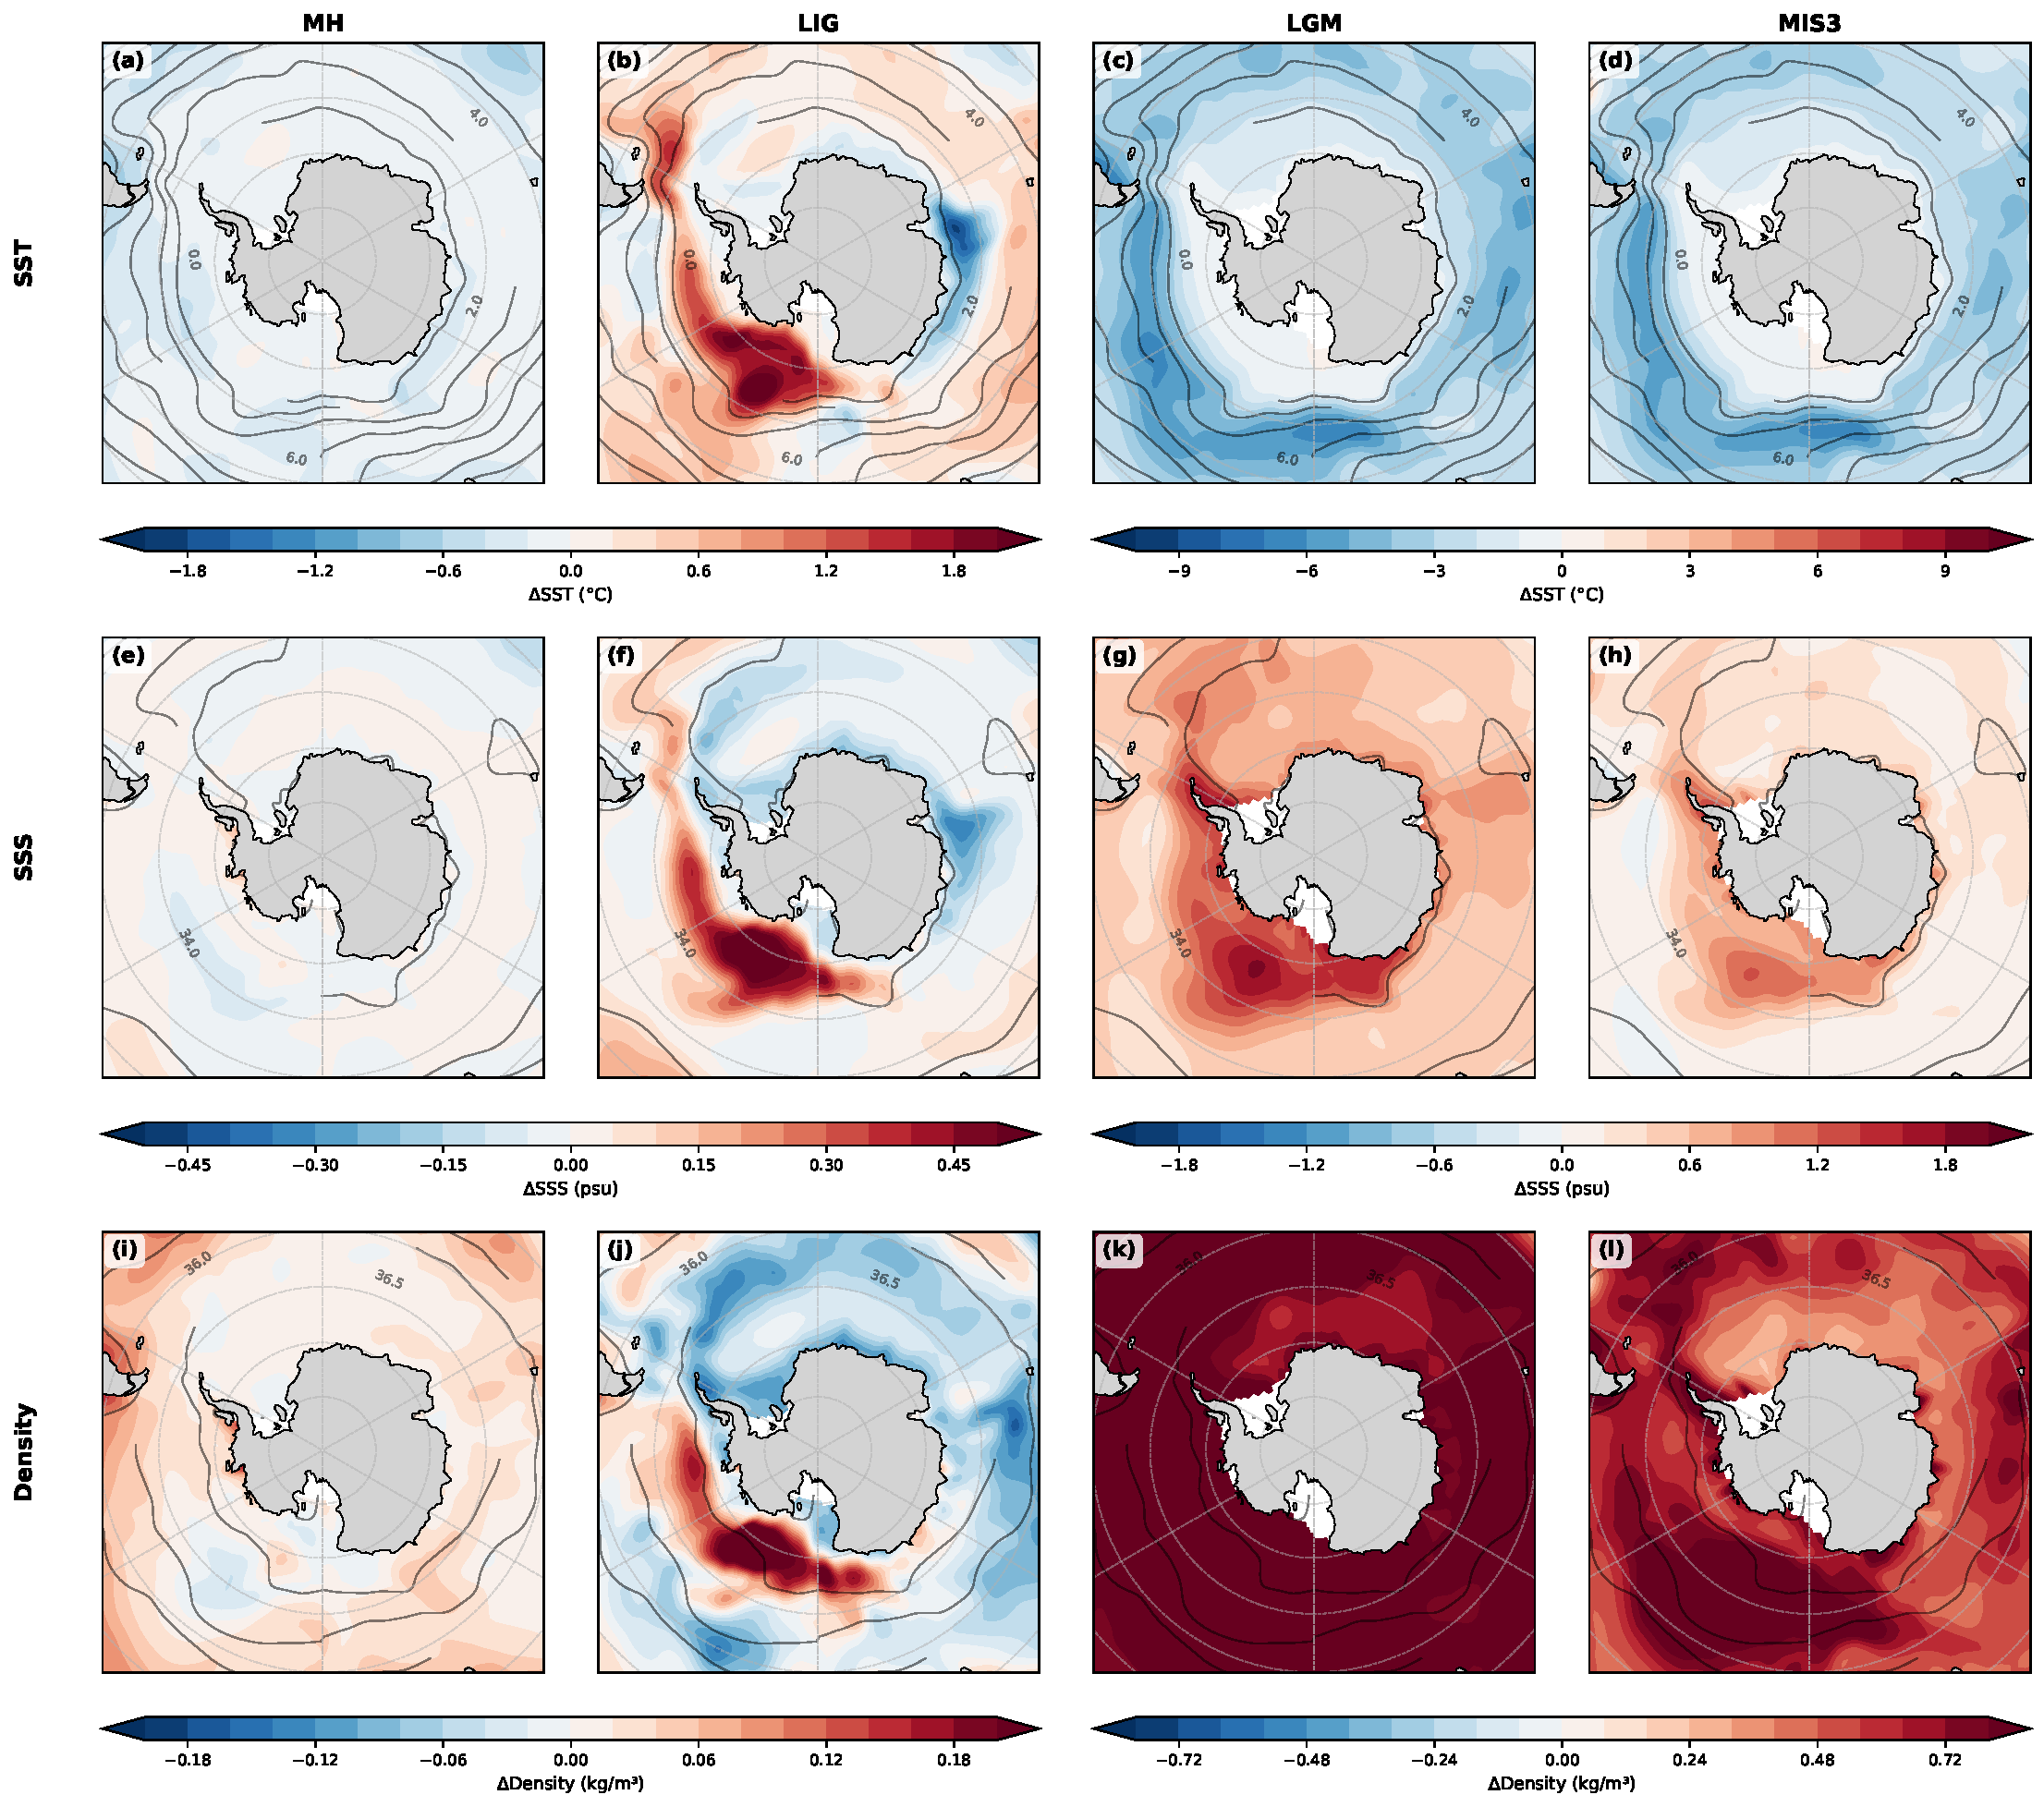
\includegraphics[width=\textwidth]{figures/fig01_climate_sst_sss_density_jja.pdf}
\end{figure}
Panel structure: 3 rows (SST, SSS, density) × 5 columns (PI absolute, MH/LIG/LGM/MIS3 anomalies). Column 1 shows PI absolute values with overlaid wind vectors; columns 2--5 show paleoclimate anomalies (paleo minus PI) in shading with PI wind contours. (a--e) Sea surface temperature (SST) in °C. LIG exhibits warming in Bellingshausen-Amundsen Seas; glacials show basin-wide cooling $>$5°C. (f--j) Sea surface salinity (SSS) in psu. Glacials display widespread salinification up to 2~psu driven by expanded sea ice. (k--o) Surface density (σ$_2$) in kg/m$^3$. Glacial periods show substantially denser surface waters (Δρ $>$ 0.6 kg/m$^3$) particularly in Atlantic and Indian sectors, reflecting combined thermal and haline effects that drive AABW precursor water formation.

\textbf{Figure 2: Sea ice extent and mixed layer depth during austral winter (JJA).}
\begin{figure}[h]
\centering
\includegraphics[width=\textwidth]{figures/fig02_climate_mld_seaice_jja.pdf}
\end{figure}
Panel structure: 2 rows (MLD, sea ice) × 5 columns. (a--e) Winter mixed layer depth (MLD) in meters for each experiment. PI/MH/LIG show 200--400~m MLD in polynyas; glacials exceed 500~m in Atlantic sector consistent with enhanced convection. (f--j) Sea ice concentration (fraction 0--1). Glacial simulations display circumpolar coverage extending to $\sim$50°S; LIG shows reduced extent compared to PI, particularly in Ross and Weddell Seas. These dramatic inter-period differences in sea ice and convective depth directly modulate AABW formation mechanisms.

\textbf{Figure 3: Wind patterns and wind stress during austral winter (JJA).}
\begin{figure}[h]
\centering
\includegraphics[width=\textwidth]{figures/fig03_climate_winds_jja.pdf}
\end{figure}
Panel structure: 2 rows × 4 columns. (a--d) 10-m wind speed anomalies (m/s) for MH/LIG/LGM/MIS3 relative to PI, with PI wind vectors overlaid. (e--h) Wind stress anomalies (N/m$^2$) with PI wind stress vectors. LIG shows poleward-shifted, strengthened westerlies (Δτ $>$ 0.04 N/m$^2$ in 50--60°S band). Glacials exhibit equatorward-shifted, weakened westerlies with widespread stress reduction. These atmospheric circulation changes directly modulate Ekman upwelling and polynya ventilation efficiency, contributing to altered AABW formation pathways.

\textbf{Figure 4: Surface heat flux components during austral winter (JJA).}
\begin{figure}[h]
\centering
\includegraphics[width=\textwidth]{figures/surface_heat_budget_anomalies_jja.pdf}
\end{figure}
Panel structure: 3 rows × 5 columns. Column 1 shows PI absolute values; columns 2--5 show paleoclimate anomalies (paleo minus PI). All heat fluxes shown from ocean's perspective (negative values indicate heat loss to atmosphere). (a--e) Total heat flux combining all atmospheric heat exchange processes (SW+LW+LH+SH). Red indicates ocean cooling (heat loss to atmosphere); blue indicates reduced cooling relative to PI. (f--j) Radiative component (SW+LW) isolating shortwave and longwave radiation contributions. (k--o) Turbulent component (LH+SH) isolating latent and sensible heat fluxes. Units: kJ~s$^{-1}$~m$^{-2}$. Glacial periods (LGM, MIS3) show dramatically reduced ocean heat loss due to sea ice thermal insulation, with turbulent flux reduction exceeding radiative changes. This paradoxical ocean warming (less cooling) despite colder atmospheric temperatures reflects expanded sea ice blocking ocean-atmosphere turbulent heat exchange.

\textbf{Figure 5: Surface heat flux components during austral summer (DJF).}
\begin{figure}[h]
\centering
\includegraphics[width=\textwidth]{figures/surface_heat_budget_anomalies_djf.pdf}
\end{figure}
Same structure as Fig.~4 but for austral summer (December-January-February). The sea ice insulation effect persists during summer in glacial ice-covered sectors, though with reduced magnitude compared to winter. Summer patterns confirm that the thermal insulation mechanism is intrinsic to ice cover rather than a winter-only phenomenon, operating year-round with seasonal modulation.

\textbf{Figure 6: Surface freshwater/mass flux components during austral winter (JJA).}
\begin{figure}[h]
\centering
\includegraphics[width=\textwidth]{figures/surface_freshwater_budget_anomalies_jja.pdf}
\end{figure}
Panel structure identical to Fig.~4. (a--e) Total freshwater flux showing net surface mass exchange. Blue indicates freshwater gain (ocean freshening); red indicates freshwater loss (ocean salinification). (f--j) Sea ice component isolating brine rejection during freezing (red: salinity increase) and freshwater release during melting (blue: salinity decrease). (k--o) Other freshwater sources (P+E+R+S) combining precipitation, evaporation, runoff, and snowfall. Units: kg~s$^{-1}$~m$^{-2}$. Glacial periods show intensified coastal brine rejection (red in panels i,j row 2) coinciding with reduced offshore ice melt, enhancing haline forcing of dense water formation in coastal polynyas. The spatial partitioning of sea ice effects---coastal intensification combined with offshore reduction---drives the shift to haline-enhanced AABW formation mechanisms during glacials.

\textbf{Figure 7: Surface freshwater/mass flux components during austral summer (DJF).}
\begin{figure}[h]
\centering
\includegraphics[width=\textwidth]{figures/surface_freshwater_budget_anomalies_djf.pdf}
\end{figure}
Same structure as Fig.~6 but for austral summer. The seasonal cycle reverses: sea ice formation in winter (Fig.~6f: positive salt tendency, red) transitions to sea ice melt in summer (Fig.~7f: negative salt tendency, blue), releasing freshwater back to the ocean. Glacial anomalies (Fig.~7i,j) show \textit{reduced} summer ice melt compared to PI (less negative values), meaning suppressed freshwater release. This asymmetry---enhanced winter brine rejection combined with reduced summer freshwater release---creates net annual haline forcing that enhances glacial AABW formation. The expanded glacial ice pack acts as a seasonal freshwater reservoir, amplifying the annual salinity cycle.

\textbf{Figure 8: Water mass transformation (WMT) in density space - annual mean.}
\begin{figure}[h]
\centering
\includegraphics[width=0.9\textwidth]{figures/plot_wmt_4regions_5exps_annual.pdf}
\end{figure}
Annual mean WMT rates (Sv) as a function of σ$_2$ density for four Southern Ocean regions: Southern Ocean (sum of all), Ross Sea, Weddell Sea, and Adélie Land. Each panel shows 5 experiments (PI, MH, LIG, LGM, MIS3). Lines indicate: total WMT (black), total heat flux contribution (red), sea ice freshwater contribution (teal), and other freshwater sources (blue). Interglacials show thermal dominance (85--90\% heat flux) at σ$_2$ = 36.6--36.8 kg/m$^3$ with modest sea ice contribution (<15\%). Glacials shift to higher densities (σ$_2$ = 37.0--37.5 kg/m$^3$) with enhanced sea ice forcing (25--30\% of total), reflecting the mechanism transition from heat-dominated to haline-enhanced AABW formation.

\textbf{Figure 9: Water mass transformation (WMT) in density space - winter mean.}
\begin{figure}[h]
\centering
\includegraphics[width=0.9\textwidth]{figures/plot_wmt_4regions_5exps_winter.pdf}
\end{figure}
Same structure as Fig.~8 but for austral winter (JJA) when AABW formation is most vigorous. Winter WMT amplitudes exceed annual means by factor of 2--3, with Southern Ocean peaks reaching 40--60~Sv (interglacials) to >60~Sv (glacials). The relative importance of sea ice forcing increases during winter, particularly in glacial periods where coastal polynya brine rejection drives 25--30\% of total transformation. Regional patterns show Weddell Sea as primary formation site (strongest glacial intensification), while Adélie Land maintains persistent heat-flux-driven transformation across all climate states.

\textbf{Figure 10: Ideal age at 3900~m depth across paleoclimate states.}
\begin{figure}[h]
\centering
\includegraphics[width=\textwidth]{figures/age_horizontal_3900m.pdf}
\end{figure}
Horizontal distribution of ideal age (years) at 3900~m depth for five experiments. Interglacials (PI/MH/LIG) exhibit young ages (0--500~yr) in Atlantic/Indian sectors with oldest waters (>1000~yr) in Pacific. Glacials (LGM/MIS3) show dramatically older ages: Atlantic/Indian exceed 1500~yr, Pacific reaches 2000--2500~yr. This represents ~1500-year global increase in deep ocean isolation, consistent with radiocarbon proxy reconstructions. Spatial patterns reflect reduced AABW formation rates and enhanced stratification under glacial boundary conditions.

\textbf{Figure 11: Ideal age anomalies at 3900~m depth.}
\begin{figure}[h]
\centering
\includegraphics[width=\textwidth]{figures/age_horizontal_3900m_anomaly.pdf}
\end{figure}
Age anomalies (years) at 3900~m for paleoclimate states relative to PI. MH shows minimal changes (±50~yr). LIG reveals younger ages (up to -150~yr) in Ross Sea sector attributed to reduced sea ice and enhanced thermal forcing, with modest increases (+50~yr) in Weddell Sea. Glacials display spatially coherent increases: LGM/MIS3 show +400 to +1500~yr across all basins, with maximum values in deep Pacific where sluggish circulation compounds the aging effect. Regional heterogeneity highlights sensitivity to local changes in surface forcing and circulation pathways.

\textbf{Figure 12: Vertical profiles of ideal age by ocean basin.}
\begin{figure}[h]
\centering
\includegraphics[width=0.8\textwidth]{figures/age_vertical.pdf}
\end{figure}
Basin-averaged vertical age profiles (years vs depth) for Atlantic, Indian, and Pacific oceans across five experiments. Interglacials show modest depth-increasing ages: Atlantic/Indian 500--750~yr at 4000~m, Pacific 800--1200~yr. Glacials exhibit systematically older ages with strong depth dependence: Atlantic reaches 1500--2000~yr, Pacific exceeds 2500~yr below 3000~m (tripling relative to PI). Indian Ocean shows intermediate behavior. These profiles quantify basin-specific ventilation changes and demonstrate that Pacific deep waters experience most dramatic aging under glacial conditions due to remoteness from AABW formation regions.

\textbf{Figure 13: Vertical profiles of ideal age anomalies by ocean basin.}
\begin{figure}[h]
\centering
\includegraphics[width=0.8\textwidth]{figures/age_vertical_anm.pdf}
\end{figure}
Basin-averaged age anomaly profiles (years vs depth, relative to PI). MH exhibits minimal anomalies (<±100~yr). LIG shows slight rejuvenation in Atlantic (-75 to -150~yr throughout water column) from enhanced AABW formation, while Pacific shows modest increases (+100~yr deep). Glacials display depth-increasing anomalies: LGM/MIS3 reach +1500~yr in deep Pacific, +800~yr in Atlantic, +500~yr in Indian. The systematic depth-dependence reflects reduced ventilation at depth where sluggish abyssal circulation magnifies the impact of reduced AABW formation rates. These anomaly profiles isolate pure climate-driven ventilation changes independent of baseline circulation structure.

% ============================================================================
% Acknowledgments
% ============================================================================
\section*{Acknowledgments}
This research was supported by... We acknowledge helpful discussions with...

% ============================================================================
% Bibliography
% ============================================================================
% This command includes your ref.bib file
% Make sure ref.bib is in the same directory as this .tex file
\bibliography{ref}

% ============================================================================
% HOW TO COMPILE:
% ============================================================================
% Run the following commands in order:
% 1. pdflatex manuscript.tex
% 2. bibtex manuscript
% 3. pdflatex manuscript.tex
% 4. pdflatex manuscript.tex
%
% Or use your LaTeX editor's "Build" button which usually does this automatically
% ============================================================================

\end{document}
